\documentclass[./Protokollheft.tex]{subfiles}
\begin{document}
\chapter{Elektrostatik und Magnetostatik 1}
%--------------- Start Vorbereitungsaufgaben ---------------
\section{Vorbereitungsaufgaben}

{\subsection{Elektrostatik}}

% --> Aufgabe
\begin{framed}
	\noindent \textbf{1.} An welchen Stellen im Gitter sind jeweils die elektrischen
Spannungen $\efit$, die Potentiale $\varphi$, die Ladungen $q$ und die
dielektrischen Flüsse $\dfit$ in der Elektrostatik allokiert?\label{exer:allocateElectrical}
\end{framed}

%%%%%%%%%%%%%%%%%%%%%%%%%%%% Antwort VB 1 %%%%%%%%%%%%%%%%%%%%%%%%%%%%%%%%%%

In der Elektrostatik sind die physikalischen Größen folgendermaßen allokiert:
\begin{itemize} 
\item elektrischen Spannungen $\efit$ auf den Kanten des primären Gitters
\item Potentiale $\varphi$ auf den Knoten des primären Gitters
\item Ladungen $q$ in den Zellen des dualen Gitters
\item dielektrischen Flüsse $\dfit$ auf den Flächen des dualen Gitters
\end{itemize}

% --> Aufgabe
\begin{framed}
	\noindent \textbf{2.} Machen Sie sich anhand einer lokalen \emph{zweidimensionalen}
Betrachtung die Beziehung zwischen der Ladung $q_n$ einer dualen Zelle $n$ und
den assoziierten Potentialen klar. Skizzieren
Sie dazu zunächst das lokale Gaußsche Gesetz für eine duale
Zelle. Nutzen Sie dabei anstatt der auftretenden Feldkomponenten 
die diskreten Potentialwerte, die Sie durch Gradientenbildung aus den 
Feldkomponenten erhalten (siehe Gleichung (4.11)).\\
Betrachten Sie dazu zunächst ein äquidistantes Gitter mit
Schrittweite $\Delta s$ und eine homogene Materialverteilung mit der
Permittivität $\eps_0$. Tragen Sie den entstehenden
"`Differenzenstern"' (Differenzen der beteiligten Potentialwerte,
die mit den Kopplungskoeffizienten gewichtet werden) in Ihre
Skizze ein.\label{exer:diffStar}
\end{framed}

%%%%%%%%%%%%%%%%%%%%%%%%%%%% Antwort VB 2 %%%%%%%%%%%%%%%%%%%%%%%%%%%%%%%%%%

Eine beliebige duale Zelle $i$ besitzt die Ladung $q_i$. Das Lokale Gaußsche Gesetz (Gleichung (4.11)) sieht dann lokal folgendermaßen aus:

\begin{align}
	\left(\divdfit\divdfit^\intercal\right)_{i,\bullet}\Phi = \left( \left(\mathbf{P}_x^\intercal\mathbf{P}_x\right)_{i,\bullet} + \left(\mathbf{P}_y^\intercal\mathbf{P}_y\right)_{i,\bullet} + \left(\mathbf{P}_z^\intercal\mathbf{P}_z\right)_{i,\bullet} \right)\Phi=\frac{1}{\Delta s \eps}\mathbf{q}_i
\end{align}

Wir nehmen ein zweidimensionales Gebiet an und die Matrizen $\mathbf{P}_{\xi}(\xi=x,y)$ definiert wie im Theorieteil von Versuch 2. Dann ergibt sich für alle $\mathbf{q}_n$, die sich nicht am Rand des Rechengebiets befinden:



\begin{align}
\begin{split}
	\left(2\cdot\Phi_n - \Phi_{n+M_x} - \Phi_{n-M_x} \right) 
+ 	\left(2\cdot\Phi_n - \Phi_{n+M_y} - \Phi_{n-M_y} \right)  
&=	\frac{1}{\Delta s \eps}\mathbf{q}_n \\ 
\Leftrightarrow 	\left(\Phi_n - \Phi_{n+M_x}\right) + \left(\Phi_n - \Phi_{n-M_x} \right) 
+ 	\left(\Phi_n - \Phi_{n+M_y}\right) + \left(\Phi_n - \Phi_{n-M_y} \right)  
&=	\frac{1}{\Delta s \eps}\mathbf{q}_n \\ 
\end{split}
\end{align}
mit $M_x=1,\,M_y=N_x$

Zur Anschauung ist auf der Abbildung \ref{img:V4.Gitter1} für eine beliebige Zelle $n$ mit Ladung $\mathbf{q}_n$ der \grqq{}Differenzenstern\grqq{}  der entsprechenden Potentiale eingezeichnet. 

\begin{figure}
\begin{center}
\begin{tikzpicture}[scale = 0.6]
%
%\pgfdeclarelayer{bg}    % declare background layer
%\pgfsetlayers{bg,main}  % set the order of the layers (main is the standard layer)
%Koordinaten & Knoten
	\coordinate (origin) at (-0.5,-0.5);
	
\def \t {1.2}
	
	\coordinate (c1) at (1*\t,1*\t);
	\coordinate (c2) at (3*\t,1*\t);
	\coordinate (c3) at (5*\t,1*\t);
	\coordinate (c4) at (7*\t,1*\t);
	\coordinate (c5) at (9*\t,1*\t);
	
	\coordinate (c6) at (1*\t,3*\t);
	\coordinate (c7) at (3*\t,3*\t);
	\coordinate (c8) at (5*\t,3*\t);
	\coordinate (c9) at (7*\t,3*\t);
	\coordinate (c10) at (9*\t,3*\t);
	
	\coordinate (c11) at (1*\t,5*\t);
	\coordinate (c12) at (3*\t,5*\t);
	\coordinate (c13) at (5*\t,5*\t);
	\coordinate (c14) at (7*\t,5*\t);
	\coordinate (c15) at (9*\t,5*\t);
	
	\coordinate (c16) at (1*\t,7*\t);
	\coordinate (c17) at (3*\t,7*\t);
	\coordinate (c18) at (5*\t,7*\t);
	\coordinate (c19) at (7*\t,7*\t);
	\coordinate (c20) at (9*\t,7*\t);	
	
%	\coordinate (c21) at (1,9);
%	\coordinate (c22) at (3,9);
%	\coordinate (c23) at (5,9);
%	\coordinate (c24) at (7,9);
%	\coordinate (c25) at (9,9);	
	
	
 
	\coordinate (d1) at (1*\t,1);	
	\coordinate (d2) at (2*\t,1*\t);
	\coordinate (d3) at (4*\t,1*\t);
	\coordinate (d4) at (6*\t,1*\t);
	\coordinate (d5) at (8*\t,1*\t);	
	\coordinate (d6) at (9*\t,1*\t);
		
	\coordinate (d7) at (1*\t,2*\t);	
	\coordinate (d8) at (2*\t,2*\t);
	\coordinate (d9) at (4*\t,2*\t);
	\coordinate (d10) at (6*\t,2*\t);
	\coordinate (d11) at (8*\t,2*\t);
	\coordinate (d12) at (9*\t,2*\t);
	
	\coordinate (d13) at (1*\t,4*\t);
	\coordinate (d14) at (2*\t,4*\t);
	\coordinate (d15) at (4*\t,4*\t);
	\coordinate (d16) at (6*\t,4*\t);
	\coordinate (d17) at (8*\t,4*\t);
	\coordinate (d18) at (9*\t,4*\t);
	
	\coordinate (d19) at (1*\t,6*\t);
	\coordinate (d20) at (2*\t,6*\t);
	\coordinate (d21) at (4*\t,6*\t);
	\coordinate (d22) at (6*\t,6*\t);
	\coordinate (d23) at (8*\t,6*\t);
	\coordinate (d24) at (9*\t,6*\t);
	
	\coordinate (d25) at (1*\t,7*\t);
	\coordinate (d26) at (2*\t,7*\t);
	\coordinate (d27) at (4*\t,7*\t);
	\coordinate (d28) at (6*\t,7*\t);
	\coordinate (d29) at (8*\t,7*\t);
	\coordinate (d30) at (9*\t,7*\t);
	
	\coordinate (legend) at (11*\t,7*\t); 
	
%	\coordinate (d31) at (1,9);
%	\coordinate (d32) at (2,9);
%	\coordinate (d33) at (4,9);
%	\coordinate (d34) at (6,9);
%	\coordinate (d35) at (8,9);
%	\coordinate (d36) at (9,9);
	
	\coordinate (fieldorigin) at (c13);

%Achsen
	\draw [->] (origin) -- ++(2,0) node [below] {$x$};
	\draw [->] (origin) -- ++(0,2) node [left] {$y$};


 
 
 
 % qn und phin
% \begin{pgfonlayer}{main} 
%	\node [above right] at (d36) {{\scriptsize $\varphi_n$}}; 
%	\node [] at ($0.5*(d29)+0.5*(d36)$) {{\scriptsize $q_n$}}; 	
% \end{pgfonlayer} 
 \begin{pgfonlayer}{b1} 
	\fill [lightred] (d20) rectangle (d15);
 \end{pgfonlayer}{b1} 
 
 \begin{pgfonlayer}{b2} 
 	\draw [-, line width=0.5mm] (c11) -- (c13);	
 	\draw [-, line width=0.5mm] (c7) -- (c17);	
\end{pgfonlayer}{b2} 

\def \la {-5}

\def \lin {1.2}

\node [] at ($(c11)+(\la,\lin+0.5)$) {{ $\left(\Phi_n - \Phi_{n+M_y} \right)$}};
\draw [-, line width=0.2mm] ($0.5*(c12)+0.5*(c17)+(0,0)$) -- ($(c11)+(\la+2,\lin+0.5)$);

\node [] at ($(c11)+(\la,0.5)$) {{ $\left(\Phi_n - \Phi_{n-M_x} \right)$}};
\draw [-, line width=0.2mm] ($0.5*(c11)+0.5*(c12)+(0,0)$) -- ($(c11)+(\la+2,0.5)$);	

\node [] at ($(c11)+(\la,-\lin+0.5)$) {{ $\left(\Phi_n - \Phi_{n+M_x} \right)$}};
\draw [-, line width=0.2mm] ($0.5*(c12)+0.5*(c13)+(0,0)$) -- ($(c11)+(\la+2,-\lin+0.5)$);	

\node [] at ($(c11)+(\la,-\lin-\lin+0.5)$) {{ $\left(\Phi_n - \Phi_{n-M_y} \right)$}};
\draw [-, line width=0.2mm] ($0.5*(c12)+0.5*(c7)+(0,0)$) -- ($(c11)+(\la+2,-\lin-\lin+0.5)$);	

\def \ab {1.3}
\def \rig {0.0}

\node [] at ($(d27)+(\rig,\ab)$) {{ $\Phi_n$}};
\draw [-, line width=0.2mm] ($(c12)+(0.15,0.15)$) -- ($(d27)+(\rig,\ab-0.3)$);	

\node [] at ($(d27)+(\rig+1,\ab)$) {{ $\mathbf{q}_n$}};
\draw [-, red, line width=0.2mm] ($(c12)+(0.5,0.5)$) -- ($(d27)+(\rig+1,\ab-0.3)$);	 

%Primäres Gitter
	%horizontal
	\draw [-] (c1) -- (c5);	
	\draw [-] (c6) -- (c10);		
	\draw [-] (c11) -- (c15);		
	\draw [-] (c16) -- (c20);		
%	\draw [-] (c21) -- (c25);		
		
%	\node [below, blue] at (2, 1) {{\scriptsize 1}}; 
	
	\draw [-] (c1) -- (c16);
	\draw [-] (c2) -- (c17);
	\draw [-] (c3) -- (c18);
	\draw [-] (c4) -- (c19);
	\draw [-] (c5) -- (c20);
	
 
%Duales Gitter
	%horizontal
	\draw [-, red] (d7) -- (d12);	
	\draw [-, red] (d13) -- (d18);	
	\draw [-, red] (d19) -- (d24);	
%	\draw [-, red] (d25) -- (d30);
	 
	%vertikal
	
	\draw [-, red] (d2) -- (d26);
	\draw [-, red] (d3) -- (d27);
	\draw [-, red] (d4) -- (d28);
	\draw [-, red] (d5) -- (d29);

%Knoten

	\foreach \i in {1,...,20}{
    	\draw[mark=*] plot coordinates {(c\i)} ; 
    }
    
    \foreach \i in {8,9,10,11,12, 14,15,16,17,18, 20,21,22,23,24, 26,27,28,29,30}{
    	\draw[mark=*, red] plot coordinates {(d\i)} ; 
    }
	
\tikzset{
  mybackground/.style={execute at end picture={
        \begin{scope}[on background layer]
          \draw[black!15,fill=black!5,rounded corners=1ex] (c7) rectangle (c15);
%          \node[draw,fill=olive,ellipse,anchor=west,inner sep=1pt,minimum width=4ex] at (c9){#1};
        \end{scope}
    }},
}
 
	
	
%Feldursprung

%	\draw[mark=*] plot coordinates {(fieldorigin)} ;
%	\node [below right] at (fieldorigin) {{\scriptsize O}}; 
	
%	\node [red] at (11,6.5) {{ \scriptsize \begin{tabular}{cc} $i_{Mitte}=3$  \\ $j_{Mitte}=3$ \\ \end{tabular} }}; 
%	\draw [-, red] (10,6.5) -- (6.1,6.1);

 

%indizierung
%	\draw [-, red, line width=0.4mm] (d2) -- (d8);	
%	\node [below, red] at (d2) {{ \scriptsize \begin{tabular}{cc} $i_{\widetilde{y}}=1$  \\ $j_{\widetilde{y}}=1$ \\ \end{tabular} }}; 
%	\node [below, red] at (d3) {{ \scriptsize \begin{tabular}{cc} $i_{\widetilde{x}}=2$  \\ $j_{\widetilde{x}}=1$ \\ \end{tabular} }}; 
%	\node [below, red] at (d4) {{ \scriptsize \begin{tabular}{cc} $i_{\widetilde{x}}=3$  \\ $j_{\widetilde{x}}=1$ \\ \end{tabular} }}; 
%	\node [below, red] at (d5) {{ \scriptsize \begin{tabular}{cc} $i_{\widetilde{x}}=4$  \\ $j_{\widetilde{x}}=1$ \\ \end{tabular} }};  
%	\draw [-, red, line width=0.4mm] (d7) -- (d8);	
%	\node [left, red] at (d7) {{ \scriptsize \begin{tabular}{cc} $i_{\widetilde{x}}=1$  \\ $j_{\widetilde{x}}=1$ \\ \end{tabular} }}; 	
%	\node [right, red] at (d12) {{ \scriptsize \begin{tabular}{cc} $i_{\widetilde{y}}=5$  \\ $j_{\widetilde{y}}=1$ \\ \end{tabular} }}; 
	
%Legend

	\def \line {0.8}

	\draw [-] (legend) -- ($(legend)+(1,0)$);
	\draw[mark=*] plot coordinates {($(legend)+(0.5,0)$)} ; 
	\node [right] at ($(legend)+(1.3,0)$) {{ \scriptsize Primäres Gitter }};
	
	\draw [-, red] ($(legend)+(0,-\line)$) -- ($(legend)+(1,-\line)$);
	\draw[mark=*, red] plot coordinates {($(legend)+(0.5,-\line)$)} ; 
	\node [right] at ($(legend)+(1.3,-\line)$) {{ \scriptsize Duales Gitter }};
 


\end{tikzpicture} 
\caption{Differenzenstern der Ladungen in Bezug auf eine beliebige Zelle $n$. }
\label{img:V4.Gitter1}
\end{center}
\end{figure}



% --> Aufgabe
\begin{framed}
	\noindent \textbf{3.} Betrachten Sie nun den Fall nichtäquidistanter Gitter
und inhomogener Materialverteilung, also die Werte der Materialmatrix im
Differenzenstern. Veranschaulichen Sie sich die Struktur der Systemmatrix $\mathbf{A}$ mit Hilfe einer Skizze der Bandstruktur.\label{exer:bandsOfSystemMat}
\end{framed}

%%%%%%%%%%%%%%%%%%%%%%%%%%%% Antwort VB 3 %%%%%%%%%%%%%%%%%%%%%%%%%%%%%%%%%%
Die Matrix $\mathbf{A}$ ist definiert als:
\begin{align}
	\mathbf{A}=\divdfit\Meps\divdfit^\intercal
\end{align}
Die Matrix $\divdfit$ besteht im Zweidimensionalen aus den Matrizen $\mathbf{P}_x$ und $\mathbf{P}_y$ :
\begin{align}
	\divdfit=\left(\mathbf{P}_x \, \mathbf{P}_y \right)
\end{align}
Die Diagonalmatrix $\Meps$ besteht im Zweidimensionalen aus den Untermatrizen $\mathbf{M}_{\eps,x}$ und $\mathbf{M}_{\eps,y}$:
\begin{align}
\Meps = \begin{pmatrix} 
    \mathbf{M}_{\eps,x}	& 0 	 				\\
	0  	 				& \mathbf{M}_{\eps,y}	\\
    \end{pmatrix}
\end{align}
Somit kann $\mathbf{A}$ umgeschrieben werden als:

\begin{align}
\mathbf{A} =  
\begin{pmatrix} 
    \mathbf{P}_x	&	\mathbf{P}_y	\\
\end{pmatrix} 
\begin{pmatrix}
\mathbf{M}_{\eps,x}	& 0 	 				\\
0  	 				& \mathbf{M}_{\eps,y}	\\
\end{pmatrix}
\begin{pmatrix} 
    \mathbf{P}_x^\intercal	\\
	\mathbf{P}_y^\intercal	\\
\end{pmatrix} 
=
\left(\mathbf{P}_x\mathbf{M}_{\eps,x}\mathbf{P}_x^\intercal + \mathbf{P}_y \mathbf{M}_{\eps,y} \mathbf{P}_y^\intercal \right)
=\mathbf{A}_x+\mathbf{A}_y
\label{eq:V4.A1}
\end{align}
Aus Gleichung ~(\ref{eq:V4.A1}) betrachten wir nun nur den Summanden $\mathbf{A}_y$ und nehmen zur Veranschaulichung ein Gitter mit 6 Knoten und $M_y=3$.

Für die Matrix $\mathbf{P}_y$ gilt somit:
\begin{align}
\mathbf{P}_y =  
\begin{pmatrix} 
   -1	& 0 	& 0	& 1		& 0 	& 0		\\
	0  	& -1	& 0	& 0		& 1		& 0		\\
   	0	& 0		&-1	& 0		& 0		& 1		\\ 
    0	& 0		& 0	& -1	& 0		& 0		\\ 
	0	& 0		& 0	& 0		& -1 	& 0		\\
	0	& 0		& 0	& 0		& 0 	& -1	\\
\end{pmatrix} 
\end{align}
%%% ausführliche Erläuterung
Nun kann man - hier beispielhaft in $y$-Richtung - die Werte der Hauptdiagonalen der Diagonalmatrix $M_{\eps , y}$ mit den Werten $m_{\eps, y, i} \; \forall i = [1, ... n]$ indizieren, schreibt also die Einträge des $y$-Anteils der Materialmatrix in einen Vektor, der jedem der $n$ Punkte der Ebene seine Permittivität in $y$-Richtung zuordnet. Es ergibt sich im betrachteten Beispiel
\begin{align}
\mathbf{A}_y =  \mathbf{P}_y \mathbf{M}_{\eps,y} \mathbf{P}_y^\intercal = 
\begin{pmatrix} 
    m_{\eps, y, 1}+m_{\eps, y, 4}	& 0 	 				& 0						& -m_{\eps, y, 4}		& 0				& 0				\\
	0  	 				& m_{\eps, y, 2}+m_{\eps, y, 5}	& 0						& 0					& -m_{\eps, y, 5}	& 0				\\
   	0				 	& 0						& m_{\eps, y, 3}+m_{\eps, y, 6}	& 0					& 0				& -m_{\eps, y, 6}	\\
    -m_{\eps, y, 4}	 		& 0						& 0						& m_{\eps, y, 4}			& 0				& 0				\\ 
	0					& -m_{\eps, y, 5}			& 0						& 0					& m_{\eps, y, 5}		& 0				\\
	0					& 0						& -m_{\eps, y, 6}			& 0					& 0				& m_{\eps, y, 6}		\\
    \end{pmatrix}
    \; .
\end{align}
Man erkennt die Bandstruktur mit je einem Abstand von $M_y$ zwischen den Neben- und der Hauptdiagonalen. 
Allgemeiner gilt also für die Systemmatrizen $\mathbf{A}_{\xi}$ mit $\xi \in \{ x,y,z \}$ eine Bandstruktur mit Abstand $M_{\xi}$ zwischen Haupt- und Nebendiagonalen
\begin{align}
\mathbf{A}_{\xi} =
\begin{pmatrix} 
    m_{\eps, \xi, 1}+m_{\eps, \xi,1+M_\xi}	&  	 		&  				&  								&  					& -m_{\eps, \xi, 1+M_\xi}		& 				& 				\\
    	 						& \ddots	& 				& 								&	 				& 						& \ddots		& 				\\
   					 			& 			& \ddots		& 								&					& 						& 				& -m_{\eps, \xi, n}	\\ 
    					 		& 			& 				& m_{\eps, \xi, n-M_\xi}+m_{\eps, \xi, n} 	&					& 						& 				& 				\\ 
    							&  			&  				&  								&m_{\eps, \xi, n-M_\xi+1}	& 						& 				& 				\\ 
    -m_{\eps, \xi, 1+M_\xi}			& 			& 				& 								&					& \ddots				& 				& 				\\ 
    				 			& \ddots	& 				& 								&					& 						& \ddots		& 				\\ 
    				 			& 			& -m_{\eps, \xi, n}	& 								&					& 						& 				& m_{\eps, \xi, n}	\\  
\end{pmatrix}
\end{align}
und die Summation dieser Matrizen erfolgt gemäß
 \begin{align}
\mathbf{A} = \sum\limits_{\xi=1}^m \mathbf{A}_{\xi} 
 \end{align}
mit $m$ der Anzahl der Raumrichtungen. Für die Systemmatrix $\mathbf{A}$ liegt damit eine Bandstruktur vor, bei der auf der Hauptdiagonalen Summenelemente der Hauptdiagonalen der einzelnen $\mathbf{A}_{\xi}$ auftreten, während die Nebendiagonalen jeweils im Abstand von $M_{\xi}$ von der Hauptdiagonalen die Einträge der Nebendiagonalen der einzelnen $\mathbf{A}_{\xi}$ übernehmen. Folglich summieren sich die Nebendiagonalelemente mehrerer $\mathbf{A}_{\xi}$ nur bei gleicher Anzahl Punkte $n_{\xi}$ in die entsprechenden Raumrichtungen.
%, insofern die $n_{\xi}$ unterschiedlich sind.
%%% ende nachträgliche ausfürhliche Erläuterung
%Wir definieren den Vektor $\mepsyp$ so dass dieser alle Elemente auf der Hauptdiagonale der Diagonalmatrix $\mathbf{M}_{\eps,y}$ beinhaltent.
%Somit können wir den $y$-Anteil der Matrix $A$ berechnen als:
%\begin{align}
%\mathbf{A}_y =  \mathbf{P}_y \mathbf{M}_{\eps,y} \mathbf{P}_y^\intercal = 
%\begin{pmatrix} 
%    \mepsy{1}+\mepsy{4}	& 0 	 				& 0						& -\mepsy{4}		& 0				& 0				\\
%	0  	 				& \mepsy{2}+\mepsy{5}	& 0						& 0					& -\mepsy{5}	& 0				\\
%   	0				 	& 0						& \mepsy{3}+\mepsy{6}	& 0					& 0				& -\mepsy{6}	\\
%    -\mepsy{4}	 		& 0						& 0						& \mepsy{4}			& 0				& 0				\\ 
%	0					& -\mepsy{5}			& 0						& 0					& \mepsy{5}		& 0				\\
%	0					& 0						& -\mepsy{6}			& 0					& 0				& \mepsy{6}		\\
%    \end{pmatrix}
%\end{align}

%Auf diese Weise erkennen wir eine Regelmäßigkeit der Bandstruktur, sodass wir die Matrix $\mathbf{A}$ allgemein berechnen können als:
%
% \begin{align}
%\mathbf{A} = \sum\limits_{\xi=1}^m A_{\xi} 
% \end{align}
%Wobei $m$ die Anzahl der Raumrichtungen ist. Und für jede Matrix $\mathbf{A}_{\xi}$ gilt:
%\begin{align}
%\mathbf{A}_{\xi} =
%\begin{pmatrix} 
%    \mepsxi{1}+\mepsxi{1+M_\xi}	&  	 		&  				&  								&  					& -\mepsxi{1+M_\xi}		& 				& 				\\
%    	 						& \ddots	& 				& 								&	 				& 						& \ddots		& 				\\
%   					 			& 			& \ddots		& 								&					& 						& 				& -\mepsxi{n}	\\ 
%    					 		& 			& 				& \mepsxi{n-M_\xi}+\mepsxi{n} 	&					& 						& 				& 				\\ 
%    							&  			&  				&  								&\mepsxi{n-M_\xi+1}	& 						& 				& 				\\ 
%    -\mepsxi{1+M_\xi}			& 			& 				& 								&					& \ddots				& 				& 				\\ 
%    				 			& \ddots	& 				& 								&					& 						& \ddots		& 				\\ 
%    				 			& 			& -\mepsxi{n}	& 								&					& 						& 				& \mepsxi{n}	\\  
%\end{pmatrix}
%\end{align}

% --> Aufgabe
\begin{framed}
	\noindent \textbf{4.} Gegeben sei ein zweidimensionales Rechengebiet mit den
Abmessungen\footnote{Alle Größen hier und im Folgenden in SI-Einheiten.} $1.2\times 0.6$ mit        
dem Koordinatenursprung bei $(0,0)$. Es seien drei Punktladungen im
Rechengebiet mit $q_1=q_0$ am Punkt $(0.3,0.2)$,  $q_2=q_0/2$ bei
$(0.6,0.4)$, und  $q_3=q_0/4$ bei $(0.9,0.2)$ gegeben.\\
Berechnen Sie die Größe und den Ort des Ladungsschwerpunkts $q_{\text{S}}$. Das
Rechengebiet sei homogen mit $\eps_0$ gefüllt und äquidistant mit
$3 \times 4$ Gitterzellen diskretisiert. Berechnen Sie außerdem die
Potentiale der Randknoten so, dass die Problemstellung mit einer
offenen Berandung versehen ist.\label{exer:averagePointCharges}
\end{framed}

%%%%%%%%%%%%%%%%%%%%%%%%%%%% Antwort VB 4 %%%%%%%%%%%%%%%%%%%%%%%%%%%%%%%%%%
Für die Größe des Ladungsschwerpuntkts $q_s$ ergibt sich
\begin{align}
q_s=\sum\limits_{i}q_i=q_0+\frac{1}{2}q_0+\frac{1}{4}q_0=1.75q_0 \; .
\end{align}
Für die Position des Ladungsschwerpunktes $r_q$ ergibt sich
\begin{align}
r_q=\frac{1}{q_s}\sum\limits_{i}q_i 
\begin{pmatrix}
x_i \\
y_i
\end{pmatrix}
=\frac{1}{1.75q_0}
q_0
\left(
1\cdot
\begin{pmatrix}
0.3 \\
0.2
\end{pmatrix}
+
\frac{1}{2}\cdot
\begin{pmatrix}
0.6 \\
0.4
\end{pmatrix}
+
\frac{1}{4}\cdot
\begin{pmatrix}
0.9 \\
0.2
\end{pmatrix}
\right)
=
\begin{pmatrix}
0.471 \\
0.257
\end{pmatrix} \; .
\end{align}
\begin{figure}
\begin{center}
\begin{tikzpicture}[scale = 0.6]
%
%\pgfdeclarelayer{bg}    % declare background layer
%\pgfsetlayers{bg,main}  % set the order of the layers (main is the standard layer)
%Koordinaten & Knoten

	
\def \t {1}  

\def \dx {3*\t} 
\def \dy {2*\t} 


\coordinate (origin) at (0,0);

\newcounter{cA} 
\newcounter{cB}  
\newcounter{cD} 
\newcounter{cC}  

\setcounter{cA}{1}

\def \nx {4} 
\def \ny {3} 

\foreach \j in {0,...,\ny}{	
	\foreach \i in {0,...,\nx}{
	
		\def \dfd {1.2} 		
		\pgfmathtruncatemacro\ii{\dx*\i}	
		\pgfmathtruncatemacro\jj{\dy*\j}	
    	\coordinate (c\thecA) at (\ii,\jj);
    	\addtocounter{cA}{1}
    }
}
    

%Primäres Gitter
	%horizontal
	

	\foreach \i in {0,...,\ny}{
		\setcounter{cA}{1+(\nx+1)*\i}	
		\setcounter{cB}{1+(\nx+1)*\i+\nx}	
    	\draw [-]  (c\thecA)-- (c\thecB);	
 	}
 	
 	\foreach \i in {0,...,\nx}{
		\setcounter{cA}{1+\i}	
		\setcounter{cB}{1+(\nx+1)*\ny+\i}	
    	\draw [-] (c\thecA) -- (c\thecB);	
	}

%Knoten

%Achsen
	\draw [->] (origin) -- ++(\nx*\dx*1.1,0) node [below] {$x$};
	\draw [->] (origin) -- ++(0,\ny*\dy*1.1) node [left] {$y$};
	
	\node [below left] at (origin) {{\scriptsize O}}; 
	\setcounter{cA}{1+\nx}
	\node [below] at (c\thecA) {{\scriptsize 1.2}}; 
	\setcounter{cA}{1+(\nx+1)*\ny}
	\node [left] at (c\thecA) {{\scriptsize 0.6}}; 

	\foreach \i in {1,...,20}{
    	\draw[mark=*] plot coordinates {(c\i)} ; 
    }
 
	\draw[mark=*, blue] plot coordinates {(0.3*\t*10,0.2*\t*10)} node [below right] {$q_1$};
	\draw[mark=*, blue] plot coordinates {(0.6*\t*10,0.4*\t*10)} node [below right] {$q_2$};
	\draw[mark=*, blue] plot coordinates {(0.9*\t*10,0.2*\t*10)} node [below right] {$q_3$}; 
 
 	\draw[mark=*] plot coordinates {(0.471*\t*10,0.257*\t*10)} node [right] {$q_n$};
 
 
 


\end{tikzpicture} 
\caption{Ladungsverteilung und Ladungsschwerpunkt.}
\label{img:V4.Gitter2}
\end{center}
\end{figure}
Um Randbedingungen für offene Berandung einzuarbeiten, sollen nun die Potentiale an den Randpunkten des Gitters mit dem Index $i$ berechnet werden gemäß
\begin{align}
\Phi_i=\frac{q_s}{4\pi\eps_0 \lvert r_i-r_q\lvert} \; .
\end{align}
Für die kanonisch indizierte Potentialwerte am Rand ergibt sich folglich beim verwendeten Rechengebiet mit $ 1.2 \times 0.6$ unter Auslassung von Einheiten

\begin{alignat*}{4}
		\Phi_{1} &= 2.9314\cdot 10^{11}\cdot q_0 \quad
		\Phi_{2} && = 5.0952\cdot 10^{10}\cdot q_0  \quad
		\Phi_{3} &&= 5.4697\cdot 10^{10}\cdot q_0 \quad 
		\Phi_{4} &&= 3.1451\cdot 10^{10}\cdot q_0 \quad \\ 
		\Phi_{5} &= 2.0348\cdot 10^{10}\cdot q_0 \quad
		\Phi_{6} &&= 3.3152\cdot 10^{10}\cdot q_0  \quad
		\Phi_{10} &&= 2.1510\cdot 10^{10}\cdot q_0 \quad
		\Phi_{11} &&= 3.1954\cdot 10^{10}\cdot q_0 \quad  \\
		\Phi_{15} &= 2.1172\cdot 10^{10}\cdot q_0 \quad 
		\Phi_{16} &&= 1.4922\cdot 10^{10}\cdot q_0 \quad 
		\Phi_{17} &&= 1.6412\cdot 10^{10}\cdot q_0 \quad 
		\Phi_{18} &&= 1.6525\cdot 10^{10}\cdot q_0 \quad  \\
		\Phi_{19} &= 1.5182\cdot 10^{10}\cdot q_0 \quad 
		\Phi_{20} &&= 1.3196\cdot 10^{10}\cdot q_0 \quad \: .
\end{alignat*}

% --> Aufgabe
\begin{framed}
	\noindent \textbf{5.} Berechnen Sie, wenn möglich, die Kapazitäten folgender Anordnungen mithilfe von Kondensatorschaltungen. Die Abmessung soll für alle Anordnungen mit $1\times1\times1$     
angenommen werden. Dabei befinden sich die Elektroden bei $y = 0$ und $y = 1$. Wie kann Anordnung e) geändert werden, damit sie mit einer Kondensatorschaltung berechnet werden kann?
\begin{enumerate}[label=\alph*)]
\item Homogen mit Permittivität $\eps_\text{r}=1$.
\item Äquidistant längsgeschichtet mit Permittivitäten $\eps_{\text{r}1}=1$ und $\eps_{\text{r}2}=2$                    (Reihenschaltung).
\item Äquidistant quergeschichtet mit Permittivitäten $\eps_{\text{r}1}=1$ und $\eps_{\text{r}2}=2$                     (Parallelschaltung).
\item Längs- und quergeschichtet mit Permittivitäten $\eps_{\text{r}1}=1$,                      
$\eps_{\text{r}2}=2$, $\eps_{\text{r}3}=3$ und $\eps_{\text{r}4}=4$ (Reihenschaltung von Parallelschaltungen bzw. Parallelschaltung von Reihenschaltungen).
\item Homogen gefüllter Kondensator ($\eps_\text{r}=1$) mit Zick-Zack-förmiger oberer Platte. Ausgehend von einem homogenen Plattenkondensator soll die Geometrie der oberen Platte durch das Einbringen eines metallischen Quaders mit den Punkten $(0,0.5,0)$ und $(0.5,1,1)$ modelliert werden.
\end{enumerate}
\label{exer:calcCapsAnalytical}
\end{framed}

%%%%%%%%%%%%%%%%%%%%%%%%%%%% Antwort VB 5 %%%%%%%%%%%%%%%%%%%%%%%%%%%%%%%%%%
Da alle Größen als SI-Eiheiten angenommen werden, werden die Einheiten bei der Berechnung der Kapazitäten ausgelassen.

\begin{enumerate}[label=\alph*)]

\item  Für eine homogen verteilte Permittivität $\eps_r=1$ ergibt sich die Kapazität eines Kondensators mit Leiterfläche $A$ und Plattenabstand $d$ zu
\begin{align}
C_a = \eps_0\eps_r \frac{A}{d} = \eps_0\cdot 1\cdot\frac{1\cdot 1}{1} = \eps_0 = 8.854 \cdot 10^{-12}\; .
\end{align}

\item  Für längsgeschichtete Permittivität $\eps_{\text{r}1}=1$ und $\eps_{\text{r}2}=2$  ergibt sich die Kapazität entsprechend einer Reihenschaltung zu
\begin{align}
\begin{split}
C_b
&= 
\left(\frac{1}{C_{b1}} + \frac{1}{C_{b2}} \right)^{-1}
=
\left(
\frac{1}{\eps_0\eps_{r2} \frac{A}{0.5\cdot d}}
+
\frac{1}{\eps_0\eps_{r2} \frac{A}{0.5\cdot d}}
\right)^{-1}
=
\eps_0 \frac{2\cdot A}{d}
\left(
\frac{1}{\eps_{r2}}
+
\frac{1}{\eps_{r2}}
\right)^{-1} \\
&=
\eps_0 \frac{2\cdot 1\cdot 1}{1}
\left(
\frac{1}{1}
+
\frac{1}{2}
\right)^{-1}
=
\frac{4}{3}\eps_0
= 1.181 \cdot 10^{-11} \; .
\end{split} 
\end{align}
 
\item Für quergeschichtete Permittivität $\eps_{r1} = 1$ und $\eps_{r2} = 2$ ergibt sich die Kapazität entsprechend einer Parallelschaltung zu 
\begin{align}
	C_c &= C_{c1} + C_{c2}
	= \eps_0 \eps_{r1} \frac{A_1}{d} + \eps_0 \eps_{r2} \frac{A_2}{d}
	= \eps_0 \frac{0.5 \cdot A}{d} \left( \eps_{r1} + \eps_{r2} \right) 
	\\
	&= \eps_0 \frac{0.5 \cdot 1 \cdot 1}{1} \left( 1 + 2 \right)
	= \eps_0 \frac{3}{2}
	= 1.328 \cdot 10^{-11} \; .
\end{align}

\item  Für sowohl längs- als auch quergeschichtete Permittivität kann die Kapazität nicht analytisch bestimmt werden, da die Stetigkeitsbedingung an den Grenzen zwischen den Bereichen nicht mehr gegeben ist. 

\item  Für die beschriebene zackenförmige Anordung lässt sich die Kapazität ebenfalls nicht elementar analytisch lösen. Es können aber aufwendige Methoden, wie die Schwarz-Christoffel Transformation angewendet werden.

\end{enumerate}

\newpage
%
{\subsection{Skalare Magnetostatik}}

% --> Aufgabe
\begin{framed}
	\noindent \textbf{6.} An welcher Stelle im Gitter müssen die Komponenten des Gitterstroms
$\jfit$ allokiert werden (bei gegebenem Ansatz des magnetischen Skalarpotentials)?\label{exer:allocateCurrent}
\end{framed}

%%%%%%%%%%%%%%%%%%%%%%%%%%%% Antwort VB 6 %%%%%%%%%%%%%%%%%%%%%%%%%%%%%%%%%%
Gemäß dem Abschnitt \textit{Lösungsprinzip in der Magnetostatik mit einem Skalarpotential} wird die magnetische Feldkomponente $ \hfit $ auf den Kanten des primären Gitters allokiert. Da damit die Summe der eine primäre Fläche umgebenden $ \hfit $-Komponenten die magnetische Spannung darstellen, schließen sie gemäß $ \mathrm{rot} \, \vec{H} = \vec{j}$ den durch die primäre Fläche fließenden Strom ein. Da die Definition der dualen Kante gerade das Durchstoßen genau einer primären Fläche beinhaltet, wird folglich der Gitterstrom $ \jfit $ auf den primären Flächen allokiert.

% --> Aufgabe
\begin{framed}
	\noindent \textbf{7.} Berechnen Sie analytisch das magnetische Feld um einen unendlich
ausgedehnten Linienleiter und skizzieren Sie die zu erwartende
Feldverteilung.\label{exer:HfieldAroundLineConductor}
\end{framed}


%%%%%%%%%%%%%%%%%%%%%%%%%%%% Antwort VB 7 %%%%%%%%%%%%%%%%%%%%%%%%%%%%%%%%%%
Aus Symmetrie-Überlegungen eines in $z$-Richtung unendlich ausgedehnten Linienleiters folgt unter Verwendung zylindrischer Koordinaten mit dem Linienleiter auf der Achse des Zylinders das Verschwinden der partiellen Ableitungen
\begin{align*}
	\partial _z \, , \; \partial _\varphi \rightarrow 0 \; \; .
\end{align*}
Betrachtet man nun einen Kreis $A$ mit Radius $R$ um den Linienleiter und führt das Integral
	 \footnote{Implizite Vernachlässigung der Beschränkung des Definitionsbereiches von $A$ durch einen radialen Schnitt mit Aussparung der Achse und der entsprechenden Singularität aufgrund der Rotationssysmmetrie des Problems}
\begin{align*}
	\oint_A \! \mathrm{rot} \vec{H} \, \cdot \, \mathrm{d} \vec{A} = 
	\oint_A \! \vec{j} \, \cdot \, \mathrm{d} \vec{A} =
	\int_{\partial A} \! \vec{H} \, \cdot \, \mathrm{d} \vec{s}
\end{align*}
aus unter Verwendung der aus $j \, \vec{e} _z = \mathrm{rot} \vec{H} \left( r \right) \; \sim \, \partial _r \left( r H_\varphi \right) $ abgeleiteten Annahme $ \vec{H} = H \left( r \right) \; \vec{e} _\varphi $ folgt
\begin{align*}
	2 \pi R \: H \left( R \right) = I \; \; .
\end{align*}
Hieraus ergibt sich durch Einsetzen des Ansatzes und der im Definitionsbereich der Koordinaten beliebigen Wahl von $R$ die bekannte Lösung
\begin{align}
	\vec{H} \left( r \right) = \frac{I}{2 \pi \, r} \; \vec{e} _\varphi \; .
\end{align}
\label{eq:v4.va9}
Die Abnahme des Wirbelfeldes $H$ erfolgt also $ \sim r^{-1} $ und damit gemäß \\
\begin{center}
\pgfplotsset{
	ticks = none,
	standard/.style = {
		every axis x label/.style = {at = {(current axis.right of origin)}, anchor = north west},
		every axis y label/.style = {at = {(current axis.above origin)}, anchor = north east},
	}
}
%\scalebox{0.5}{

\begin{tikzpicture} %[xscale = 3.5, yscale = 2]
%	\draw [ultra thick, <->] (0,2) -- (0,0) -- (3.5,0);
	\begin{axis}[
		width = 0.4 \textwidth,
		height = 0.2 \textheight,
		axis x line = bottom,
		axis y line = left,
		xmin = 0, xmax = 3.5,
		ymin = 0, ymax = 2,
		xticklabel = \empty,
		yticklabel = \empty,
		ytick = {},
		xlabel = { $r$ },
		ylabel = { $\vert \, H \, \vert $ },
%		xlabel style = {at = {(current axis.right of origin)}},
%		ylabel style = {at = {(current axis.above origin)} anchor = south},
		]	
	\addplot [mark = none, domain = 0:3.5] { 1/x};	
	%\draw [domain = 0.5:3.5] plot (\x, {1 / \x});
	\end{axis}
\end{tikzpicture}
%}
\end{center}



% --> Aufgabe
\begin{framed}
	\noindent \textbf{8.} Wie können die Dirichlet- und die Neumann- Randbedingung physikalisch gedeutet werden, wenn sie in der Magnetostatik auf das magnetische Skalarpotential angewandt werden?\label{exer:bndCondMagScalarPot}
\end{framed}

%%%%%%%%%%%%%%%%%%%%%%%%%%%% Antwort VB 8 %%%%%%%%%%%%%%%%%%%%%%%%%%%%%%%%%%
Gemäß dem Abschnitt \textit{Randbedingungen} entsprechen Dirichlet-Randbedingungen einer Vorgabe des magnetischen Skalarpotentials $\phi _m$ auf der Berandung des Rechengebietes. Im Gegensatz dazu geben Neumann-Randbedingungen Anforderungen an den Gradienten des Skalarpotentials und damit an $ {- \mathrm{grad}} \, \phi _m = \vec{H} _h $ vor.
Analog zur Deutung  der Randbedingungen der Elektrostatik lassen sich die physikalischen Interpretationen also erkennen als:
\begin{itemize}
	\item Dirichlet: magnetisch (ideal) leitende Oberfläche
	\item Neumann: Fläche mit magnetischer Flächenladung (ggf. Dipol-Oberfläche)
\end{itemize}


% --> Aufgabe
\begin{framed}
	\noindent \textbf{9.} Das Problem eines unendlich langen Leiters ist ein
offenes 2D-Problem und müsste durch eine offene
Randbedingung in der FIT modelliert werden. Wenn das
Rechengebiet hinreichend groß ist, kann ohne großen
Genauigkeitsverlust für die Felder im Inneren des Rechengebiets
auf die komplizierte Implementierung eines offenen Randes
verzichtet werden. Welche Randbedingung eignet sich hierfür besser? (Neumann ($H_{\text{n}}=0$) oder Dirichlet ($\vec{H}_{\text{t}}=0$))?\label{exer:boundCondInfiniteConductor}
\end{framed}

%%%%%%%%%%%%%%%%%%%%%%%%%%%% Antwort VB 9 %%%%%%%%%%%%%%%%%%%%%%%%%%%%%%%%%%
Gemäß \ref{eq:v4.va9} ist das magnetische Feld im betrachteten Rechengebiet tangential an jedem Kreisbogen um die Achse. In anderen Worten: Der radiale, normal zu einer Fläche auf einem Rand in Form eines Kreisbogens stehende Anteil $H_n$ des Feldes verschwindet $H_n = 0$.  Dies legt somit die Verwendung einer neumannschen Randbedingung nahe. Diese Aussage gilt in größerem Abstand von der Achse und damit verbundener lokaler Vernachlässigung der Krümmung des Kreisbogens auch für Ränder, deren Normalen in jedem Punkt einen (wesentlich) größeren Anteil in $\vec{e} _r$- als in $\vec{e} _\varphi$-Richtung haben.


\section{Aufgaben während der Praktikumssitzung}

{\subsection{Elektrostatik}}

Kern dieses Abschnitts bildet die Implementierung eines Solvers für elektrostatische
Probleme. Anhand der Kondensatoranordnungen aus der Vorbereitung können die
Routinen mit analytischen Berechnungen verglichen und das Konvergenzverhalten
untersucht werden. Der Kondensator mit Knick dient darüber hinaus als Beispiel
für ein analytisch nicht lösbares Problem.

% --> Aufgabe
\begin{framed}
	\phantomsection \label{v4.PA.1}
	\noindent \textbf{1.} Vervollständigen Sie die in \lstinline{solveES.m} vorgegebene Funktion
\begin{align}
\lstinline{[phi, ebow, dbow, relRes] = solveES(msh, eps, pots, q, bc)} \; ,
\end{align}
welche einem allgemeinen Elektrostatik-Solver entspricht. \lstinline{msh} ist hierbei das Rechengitter, \lstinline{eps} die Permittivität, \lstinline{pots} die gesetzten Potentiale für jeden Gitterpunkt (nicht bekannte Potentiale sind mit dem Wert \lstinline{NaN} in diesem Vektor gekennzeichnet), \lstinline{q} die vorgegebenen Ladungen und \lstinline{bc} die vorgegebenen Randbedingungen. \lstinline{phi}, \lstinline{ebow} und \lstinline{dbow} sind die integralen Feldgrößen und \lstinline{relRes} ist ein Vektor mit den relativen Residuen des Solvers in jedem Iterationsschritt.\\
\ \\
{\textbf{Hinweis:}} Für die Implementierung werden Ihnen einige Routinen vorgegeben
(zum Teil handelt es sich um optimierte Funktionen aus vergangenen Versuchen), welche auf den nächsten Seiten beschrieben sind. Verwenden Sie diese so oft wie möglich.\label{exer:solveES}
\end{framed}

% --> Antwort

\textit{ Code siehe Seite \pageref{code4.1} } \\
Die Implementierung erstellt zunächst die Systemmatrix $\mathbf{A} = \mathbf{\divdfit}\mathbf{\Meps}\mathbf{\divdfit}^T$ und die dafür benötigten topologischen und geometrischen Matrizen. Anschließend werden die festgelegten Potentiale und die zugehörigen Matrixeinträge entfernt und dann das Problem $\mathbf{A}\mathbf{\phi} = \mathbf{q}$ mit Hilfe der Funktion \lstinline{pcg} gelöst.
Diese Methode nutzt einen iterativen Solver und die relativen Residuen in jedem Iterationsschritt werden in dem Feld \lstinline{relRes} gespeichert. Schlussendlich werden die bereits bekannten Potentiale mit der Lösung des Solvers zusammengeführt und die Felder $\efit$ und $\dfit$ berechnet.

% --> Aufgabe
\phantomsection \label{v4.PA.2}
\begin{framed}
	\noindent \textbf{2.} Schreiben Sie eine Methode
\begin{align}
\lstinline{cap = calcCap(msh, ebow, dbow)} \; ,
\end{align}
die die Kapazität \lstinline{cap} berechnet und zurück gibt. Verwenden Sie hierzu die vorgegebenen Methoden \lstinline{intEdge} und
\lstinline{intSurf}.\label{exer:calcCap}
\end{framed}

% --> Antwort
\textit{ Code siehe Seite \pageref{code4.2} } \\
Die Implementierung verwendet die Funktion \lstinline{intEdge} um den Spannungsabfall zwischen den Kondensatorplatten zu berechnen, indem entlang eines Weges von der unteren zur oberen Kondensatorplatte integriert wird. Anschließend wird die Gesamtladung der Anordnung bestimmt, indem über die gesamte Querschnittsfläche der Anordnung in der Mitte zwischen den Platten integriert wird. Die Kapazität folgt anschließend aus $C = \frac{Q}{U}$.

% --> Aufgabe
\phantomsection \label{v4.PA.3}
\begin{framed}
	\noindent \textbf{3.} Verwenden Sie nun die letzten beiden Methoden in dem teilweise vorgegebenen Skript \lstinline{exampleCaps.m}, um
die Kapazität der Kondensatorkonfigurationen a) bis d) der Vorbereitungsaufgaben numerisch zu berechnen und mit Ihren analytischen Ergebnissen zu vergleichen. Hängt die Lösung von der Größe des Gitters ab?\label{exer:calcCapNumerically}
\end{framed}

% --> Antwort
\textit{ Code siehe Seite \pageref{code4.3} } \\
Die Lösung ist für größere Gitter genauer, da die Geometrie mit mehr Stützstellen besser aufgelöst ist. Dies ist vor allem im Fall e) zu erkennen.
Die Implementierung erzeugt zunächst ein \lstinline{msh} und definiert mit Hilfe der Funktion \lstinline{boxMesher} die Füllungen der Zellen mit den entsprechenden Permittivitäten sowie die Randbedingungen des Gitters. Anschließend werden die Funktionen \lstinline{solveES} und \lstinline{calcCap} verwendet um die Kapazität der Anordnungen zu berechnen.

\lstinputlisting[language=Matlab, caption={Matlab-Console : Kapazitäten der Anordnungen} , label={V4.PA3Listing}, captionpos=b, numbers=none, keywordstyle=\color{black}]{versuch4/A3_console_output.txt}

Die Ergebnisse in \ref{V4.PA3Listing} decken sich mit den Erwartungen aus der Vorbereitung.

% --> Aufgabe
\phantomsection \label{v4.PA.4}
\begin{framed}
	\noindent \textbf{4.} Visualisieren Sie im selben Skript das Potential (\lstinline{plotPotential}) und das elektrische Feld (\lstinline{plotEdgeVoltage})
der fünf Kondensatorkonfigurationen. Wählen Sie hierfür eine sinnvolle Diskretisierung und eine zweidimensionale Darstellung mit sinnvoller Schnittebene~\lstinline{indz}. Kommentieren Sie kurz die Feldbilder im Hinblick auf die analytischen Feldverläufe.\label{exer:visualizeCapField}
\end{framed}

% --> Antwort
Die Implementierung ergänzt den Code der vorherigen Aufgabe um die Funktionen \lstinline{plotPotential} und \lstinline{plotEdgeVoltage}, mit deren Hilfe das Potential und das elektrische Feld dargestellt werden. In den Abbildungen \ref{fig:V4.PA4.1}, \ref{fig:V4.PA4.2} und \ref{fig:V4.PA4.3} sind die Größen für die Anordnung aus Aufgabe \ref{exer:calcCapsAnalytical} ~e) dargestellt.
\begin{figure}[htb]
\begin{center}
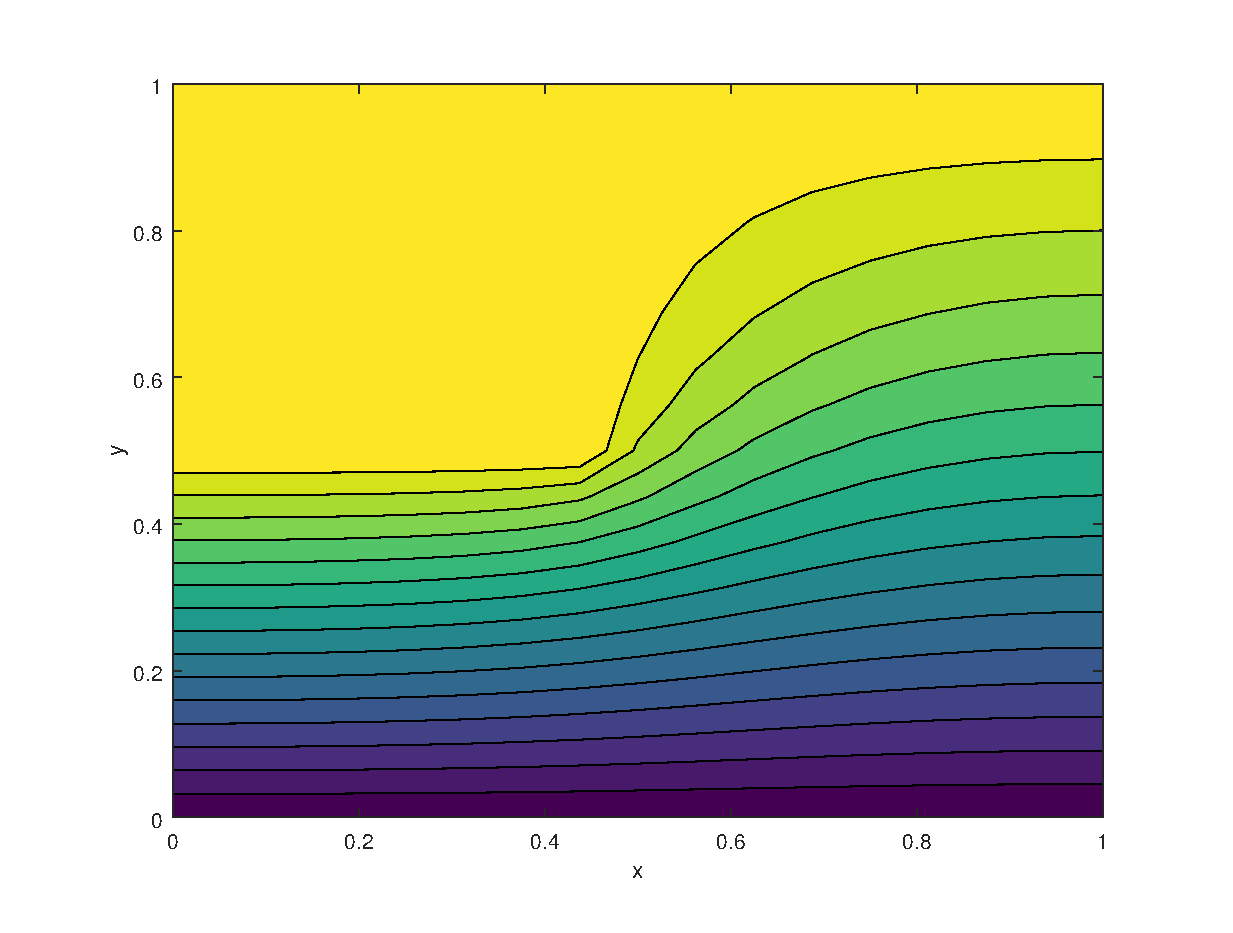
\includegraphics[scale=0.6]{eps/plotPot}
\end{center}
\caption[Potentialverlauf eines Kondensators mit Kante]{Potentialverlauf des Kondensators mit Kante.}
\label{fig:V4.PA4.1}
\end{figure}

\begin{figure}[hp]
\begin{center}
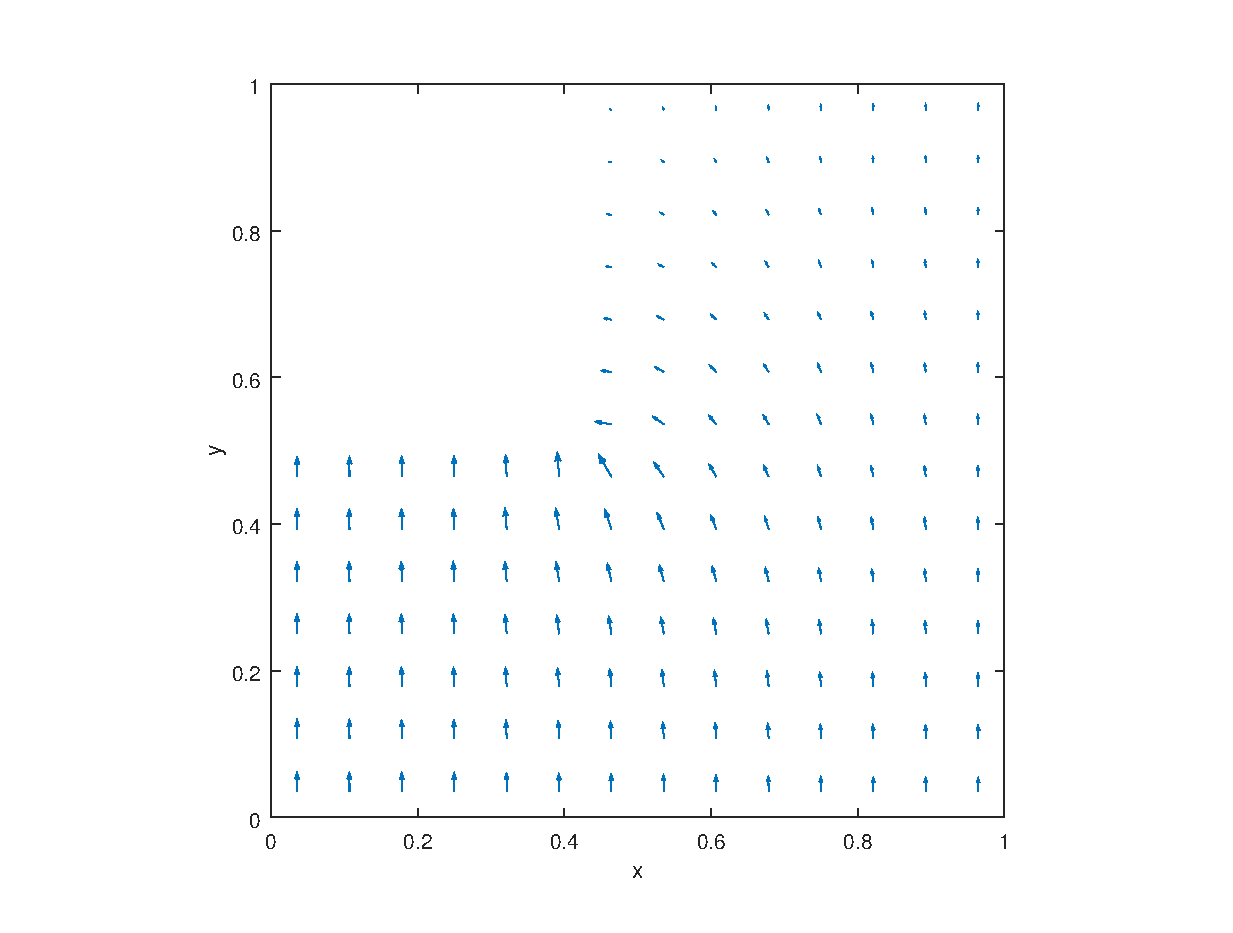
\includegraphics[scale=0.7]{eps/plotE2D}
\end{center}
\caption[E-Feld eines Kondensators mit Kante in 2D]{E-Feld des Kondensators mit Kante in 2D.}
\label{fig:V4.PA4.2}
\end{figure}

\begin{figure}[hp]
\begin{center}
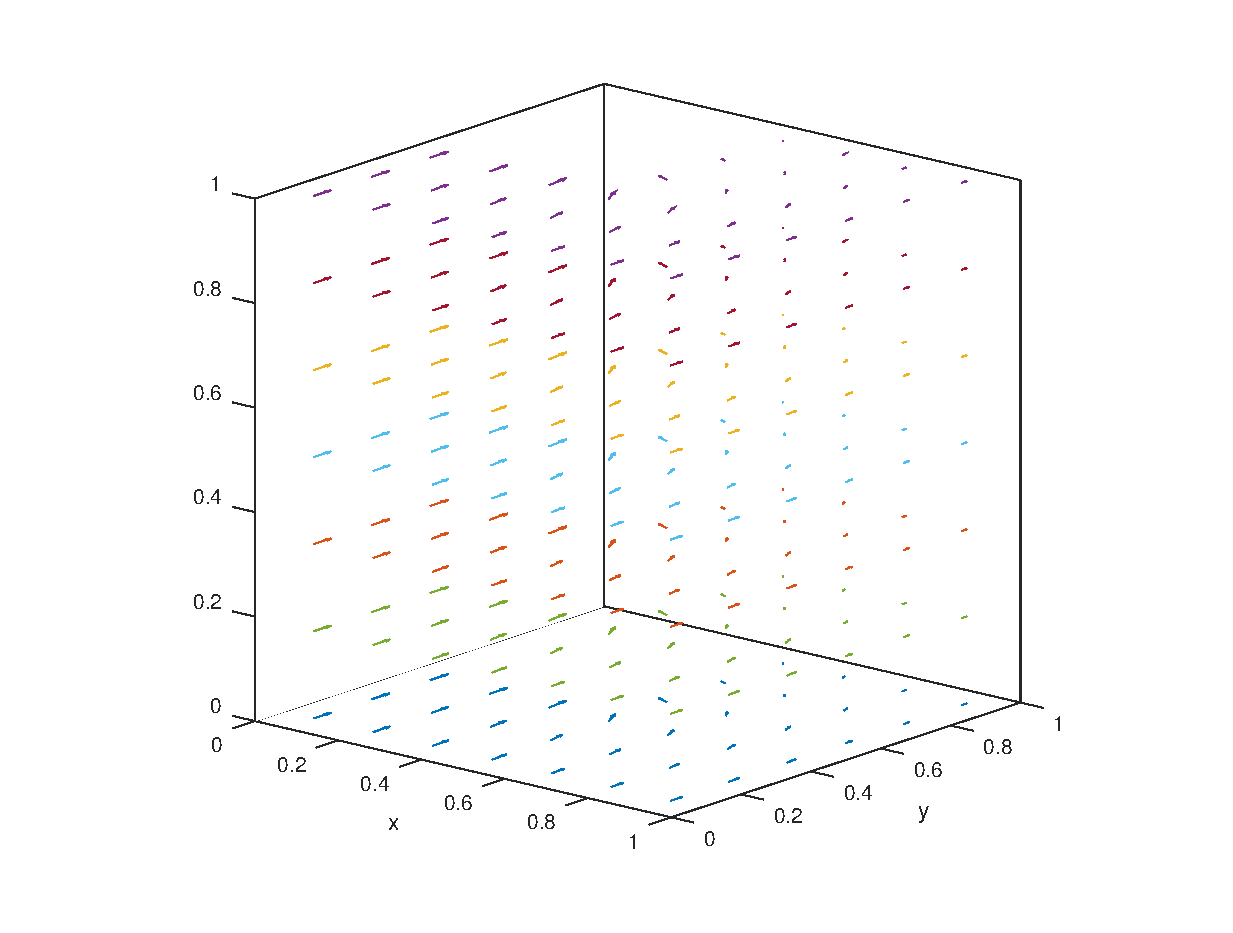
\includegraphics[scale=0.7]{eps/plotE3D}
\end{center}
\caption[E-Feld eines Kondensators mit Kante in 3D]{E-Feld des Kondensators mit Kante in 3D.}
\label{fig:V4.PA4.3}
\end{figure}

%% --> Aufgabe
\phantomsection \label{v4.PA.5}
\begin{framed}
	\noindent \textbf{5.}   Dokumentieren Sie das Konvergenzverhalten des iterativen Solvers für Kondensatorkonfiguration~e), indem Sie
den Verlauf des relativen Residuums als Funktion des Iteratonsschritts $n_\text{iter}$ mithilfe eines Matlab-Skripts \lstinline{plotConv.m} grafisch darstellen.\\
{\textbf{Hinweis:}} Entsprechend Vorgabe ist das relative Residuum für jeden Iterationsschritt in \lstinline{relRes} enthalten.\label{exer:plotCapConvSolver}
\end{framed}

% --> Antwort
\textit{ Code siehe Seite \pageref{code4.5} } \\
Die Implementierung erzeugt und löst das Problem äquivalent zu Aufgabe \ref{exer:calcCapNumerically} und plottet anschließend die relativen Residuen über der Zahl des jeweiligen Iterationsschritts. Das Konvergenzverhalten ist in Abbildung \ref{fig:V4.PA5} dargestellt.
\begin{figure}[p]
\begin{center}
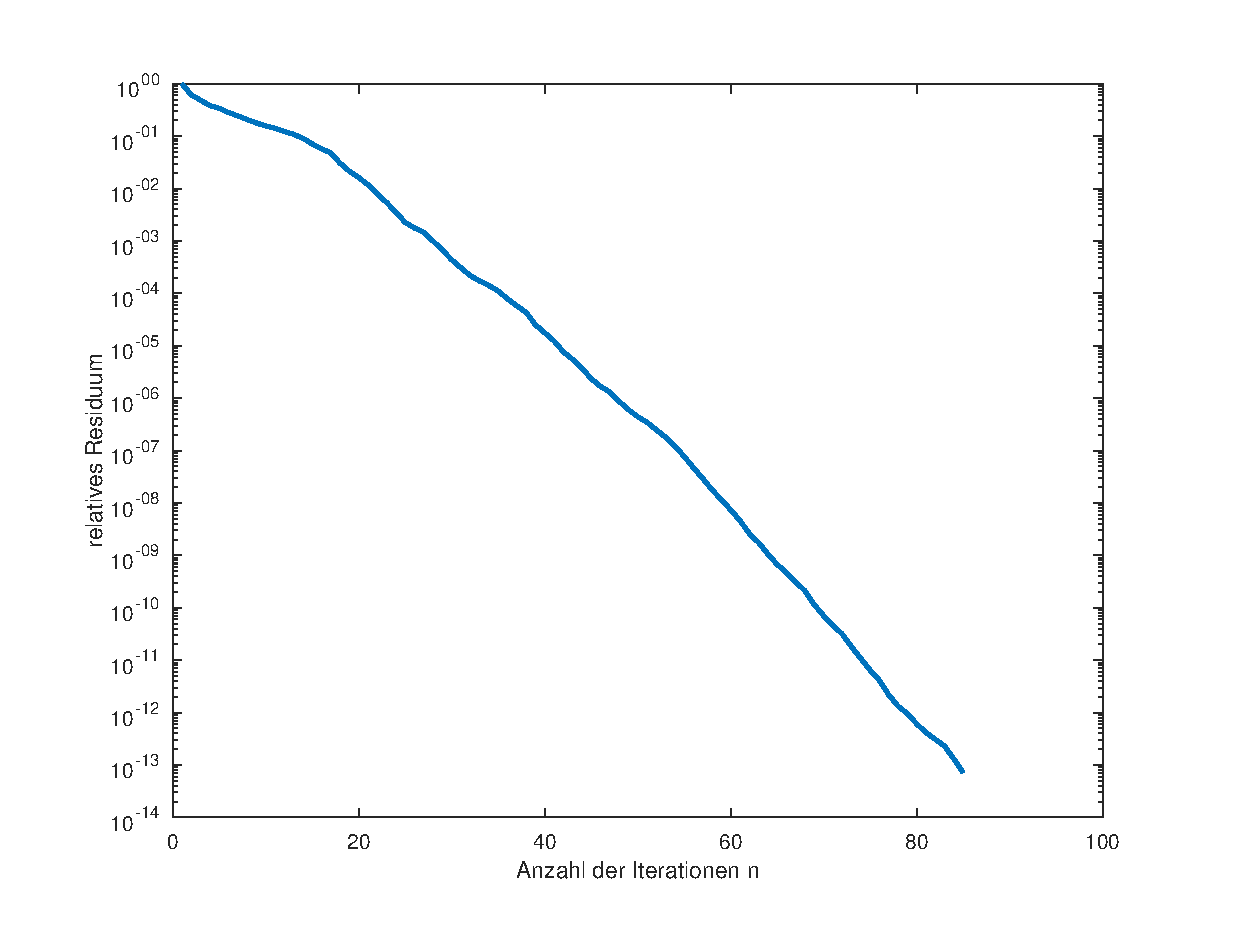
\includegraphics[scale=0.7]{eps/plotConv}
\end{center}
\caption{Konvergenzverhalten des Solvers \lstinline{pcg}.}
\label{fig:V4.PA5}
\end{figure}

% --> Aufgabe
\phantomsection \label{v4.PA.6}
\begin{framed}
	\noindent \textbf{6.} Schreiben Sie nun ein Skript \lstinline{plotConvCap.m}, das die letzte Kondensatorkonfiguration e) numerisch berechnet
und zusätzlich das Konvergenzverhalten (hier nicht vom Gleichungssystemlöser, sondern von der Gitterverfeinerung)
angibt. Stellen Sie auch diese Lösung wieder grafisch dar.\\
Welcher Unterschied besteht zwischen der Konvergenz des iterativen Solvers und der Verbesserung der Lösungsgenauigkeit durch zunehmende Gitterzellenanzahl, der sogenannten Verfahrenskonvergenz?\label{exer:plotCapConvMesh}
\end{framed}

% --> Antwort
\textit{ Code siehe Seite \pageref{code4.6} } \\
Die Implementierung arbeitet analog zu Aufgabe \ref{exer:plotCapConvSolver} und enthält eine zusätzliche Schleife, die die Anzahl der Stützstellen variiert.
Die Verfahrenskonvergenz ist in Abbildung \ref{fig:V4.PA6} dargestellt.
Die Verfahrenskonvergenz beschreibt die Konvergenz der numerischen Lösung gegen die Analytische, wobei sich die Konvergenz des Gleichungssystemslösers nur auf die bestmögliche Lösung mit der für die Matrixerzeugung genutzten Diskretisierung bezieht. Diese stimmt im Allgemeinen allerdings nicht mit der analytischen Lösung überein, da das Gitter die Geometrie nicht perfekt abbildet.
\begin{figure}[hp]
\begin{center}
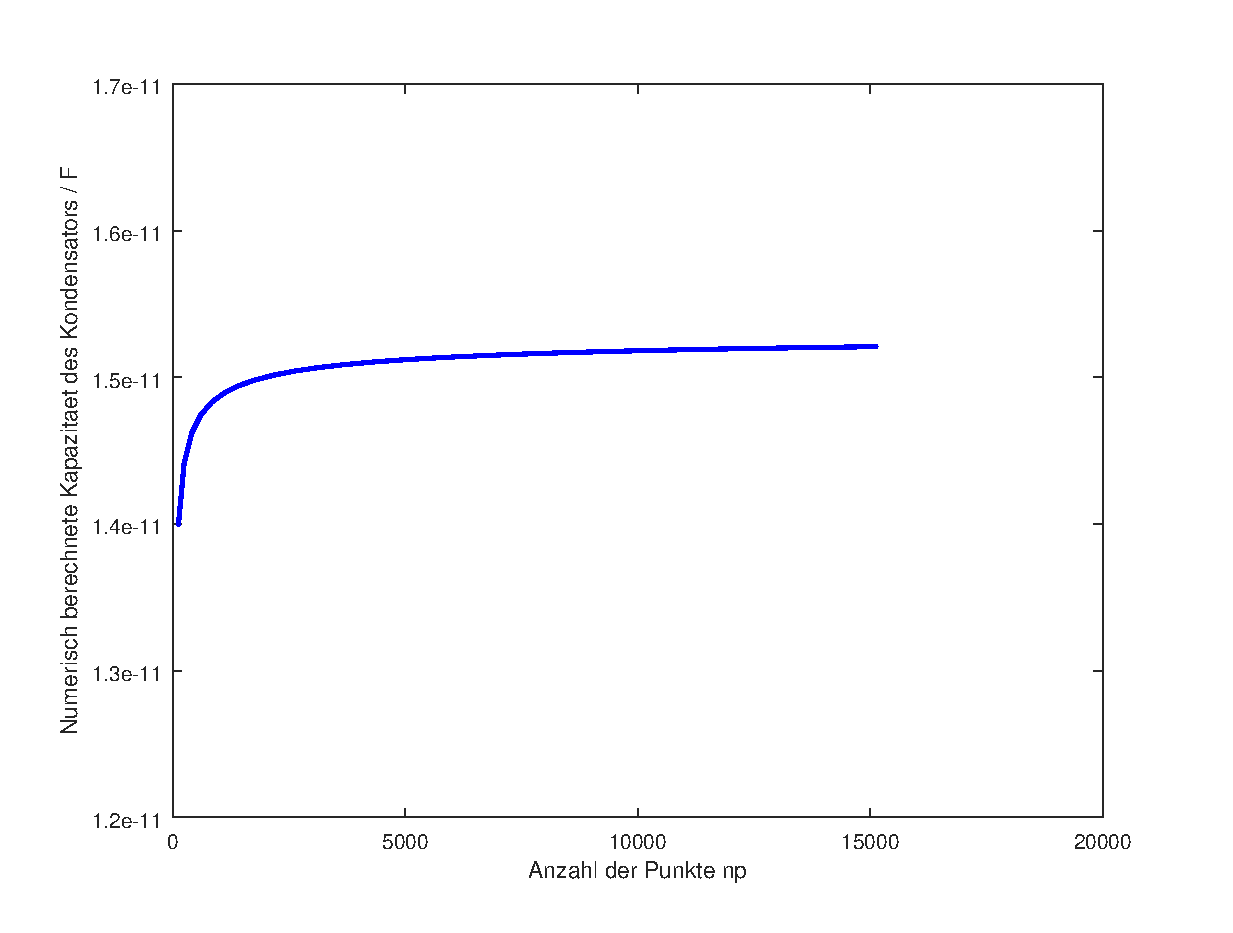
\includegraphics[scale=0.7]{eps/plotConvCap}
\end{center}
\caption{Konvergenzverhalten der Gitterverfeinerung.}
\label{fig:V4.PA6}
\end{figure}

%
{\subsection{Skalare Magnetostatik}}
Analog zur Elektrostatik wird nun ein Solver für magnetostatische Probleme implementiert, welcher das magnetische Skalarpotential verwendet. Das Rechengebiet wird erneut zu $1\times 1\times 1$ gewählt. In der Mitte des Rechengebietes soll sich ein in $z$-Richtung das komplette Rechengebiet durchlaufender Linienleiter, der den Strom \SI{1000}{A} führt, befinden.

% --> Aufgabe
\phantomsection \label{v4.PA.7}
\begin{framed}
	\noindent \textbf{7.} Verwenden Sie die vorgegebene Methode \lstinline{calcHi}, um das Hilfsfeld $\hfit_{\text{i}}$ des Linienleiters zu berechnen.
Stellen Sie es grafisch dar. Nutzen Sie für diese Implementierung bitte das gegebene Skript \lstinline{exampleHi.m}.\label{exer:visualizeHi}
\end{framed}

%%%%%%%%%%%%%%%%%%%%%%%% Antwort A 7 %%%%%%%%%%%%%%%%%%%
\textit{ Code siehe Seite \pageref{code4.7} } \\
Der Linienleiter mit $I = \SI{1000}{A}$ in $\vec{e}_z$-Richtung liegt zentral in der Mitte des Rechengebietes der xy-Ebene und bei der verwendeten ungeraden Anzahl an Punkten in $x$- und $y$-Richtung damit entlang der primären Kanten.
Folglich wird $\jfit$ gleichermaßen auf die vier an einen Punkt in der Mitte der xy-Ebene angrenzenden Flächen aufgeteilt. Damit ergeben sich die Einträge in $\jfit_z$ mit Indizes
\begin{align}
	\begin{split}
		n_1 \left( i,j,k \right) = n_{\mathrm{mid}}
			= n \left( \frac{n_x +1}{2} , \; \frac{n_y +1}{2} , \: k \right)
	\end{split}
	\\
	\begin{split}
		n_2 \left( i,j,k \right) = n_{\mathrm{mid}} - M_x
			= n \left( \frac{n_x +1}{2}-1 , \; \frac{n_y +1}{2} , \; k \right)
	\end{split}
	\\
	\begin{split}
		n_3 \left( i,j,k \right) = n_{\mathrm{mid}} - M_y
			= n \left( \frac{n_x +1}{2} , \; \frac{n_y +1}{2} -1 , \; k \right)
	\end{split}
	\\
	\begin{split}
		n_4 \left( i,j,k \right) = n_{\mathrm{mid}} - M_x - M_y
			= n \left( \frac{n_x +1}{2}-1 , \; \frac{n_y +1}{2}-1 , \; k \right)
	\end{split}
\end{align}
für alle möglichen $k$-Ebenen in $z$-Richtung.
Diesem Ausdruck entspricht die Implementierung der Methode.
\\
Das entstehende Feld in \ref{fig:V4.PA7} zeigt die prinzipielle Erwartung eines Wirbelfeldes, jedoch entspricht die unterschiedliche Wirbelstärke entlang der $x$- und $y$-Achse nicht dem erwarteten Feldbild und belegt damit die unphysikalische Eigenschaft dieses Hilfsfeldes.
\begin{figure}[h]
\begin{center}
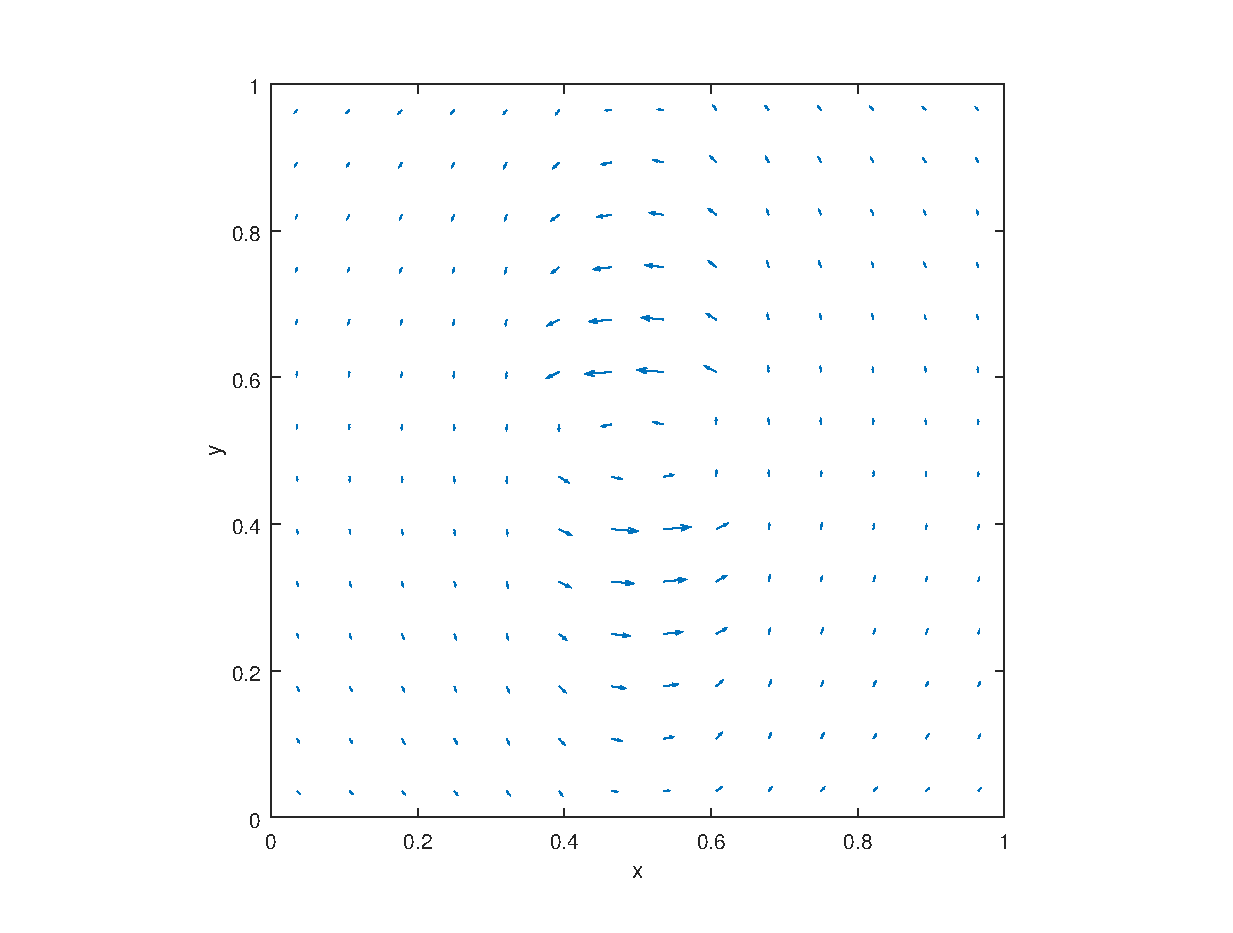
\includegraphics[scale=0.7]{eps/plotExampleHi}
\end{center}
\caption{Linienleiter mit magnetostatischem Hilfsfeld $H_i$.}
\label{fig:V4.PA7}
\end{figure}

% --> Aufgabe
\phantomsection \label{v4.PA.8}
\begin{framed}
	\noindent \textbf{8.} Vervollständigen Sie den Solver
\begin{align}
\lstinline{[hbow, bbow, relRes] = solveMS(msh, mu, jbow, bc)} \; ,
\end{align}
wobei \lstinline{mu} hier die Permeabilität, \lstinline{jbow} der Gitterstromfluss und
\lstinline{hbow} bzw. \lstinline{bbow} die Feldgrößen sind.\\
\ \\
{\textbf{Hinweis:}} Verwenden Sie wieder die vorgegebenen Routinen sowie die \matlab-Datei \lstinline{solveMS}. Benutzen Sie
dafür u.\,A. die Routine \lstinline{createMeps} und beachten Sie die vertauschte Allokation der Felder in der skalaren Magnetostatik.\label{exer:solveMS}
\end{framed}

%%%%%%%%%%%%%%%%% Antwort A 8 %%%%%%%%%%%
\textit{ Code siehe Seite \pageref{code4.8} } \\
Die Implementierung von $\lstinline{solveMS}$ in \ref{code4.8} nutzt die Implementierung der Elektrostatik aus den vorangegangenen Versuchen durch analoge Berechnungsverfahren. Dies resultiert aus der Allokation von $\hfit$ auf den primären Kanten. Es werden lediglich die magnetischen Ladungen zuerst aus dem unphysikalischen Hilfsfeld $H_i$ gemäß Aufgabe 7 berechnet.

% --> Aufgabe
\phantomsection \label{v4.PA.9}
\begin{framed}
	\noindent \textbf{9.} Verwenden Sie \lstinline{solveMS} um das $\vec{H}$-Feld zu berechnen und grafisch darzustellen. Nutzen Sie für diese Implementierung bitte das Skript \lstinline{exampleMShomogen.m}. Entspricht das Feldbild Ihren Erwartungen?\label{exer:visualizeHfield}
\end{framed}

%%%%%%%%%%%%%%%%%%%%%% Antwort A 9 $$$$$$$$$$$$$$$$$ 
\textit{ Code siehe Seite \pageref{code4.9} } \\
Die Definition des Stromvektors $\jfit$ erfolgt gemäß den Erläuterungen aus Aufgabe 7.
\\
Unter Ausnutzung von \lstinline{solveMS} berechnet sich aus dem unphysikalischen Hilfsfeld das den Erwartungen entsprechende Feldbild \ref{fig:V4.PA9} eines Linienleiters. Offensichtlich ist die rotationssymmetrische Stärke des Wirbelfeldes, auch die $ \sim r^{-1} $ verlaufende Abnahme lässt sich herauslesen. 
\begin{figure}[hp]
\begin{center}
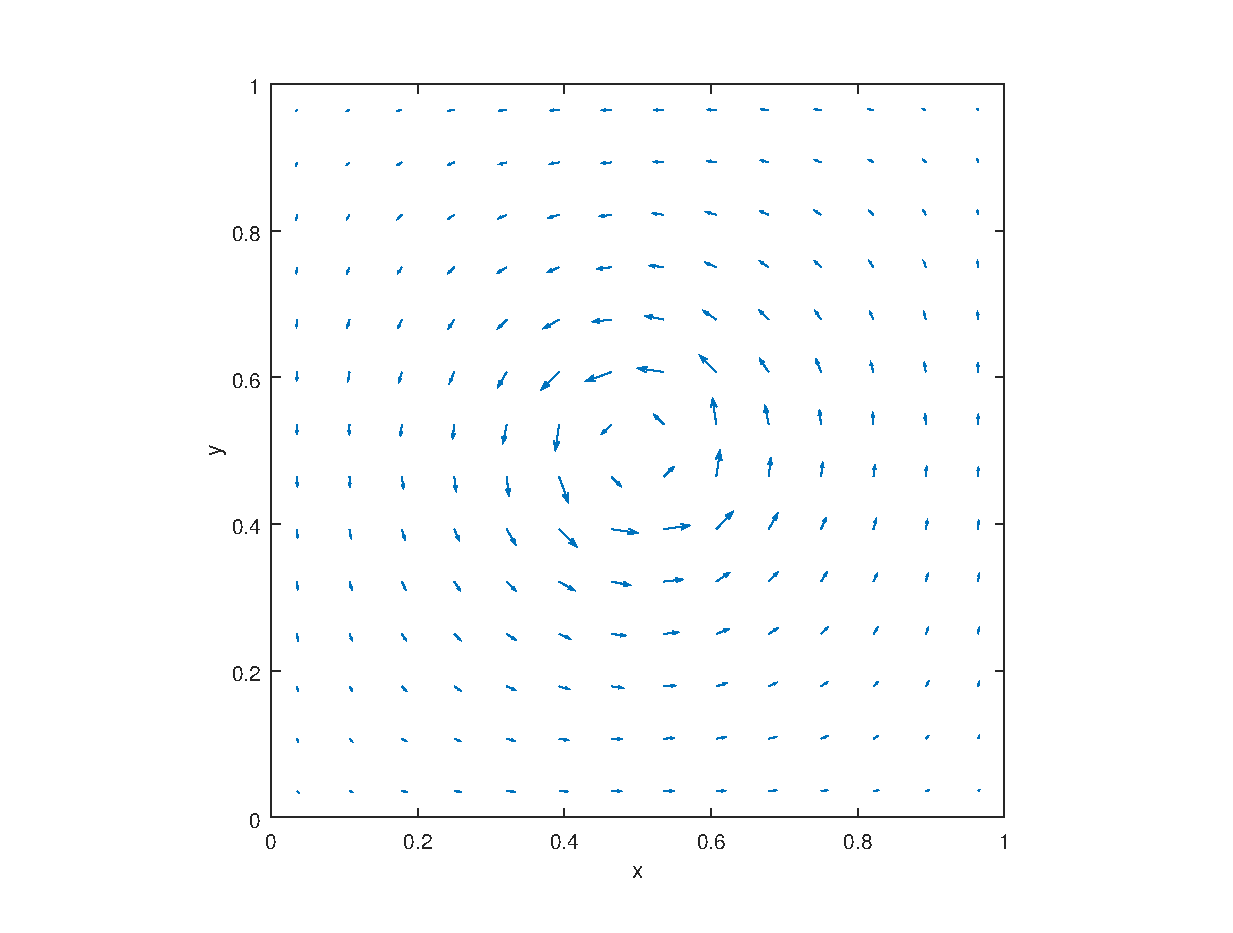
\includegraphics[scale=0.7]{eps/plotMShomogen}
\end{center}
\caption{Feldbild eines Linienleiters bei homogener Materialverteilung.}
\label{fig:V4.PA9}
\end{figure}

% --> Aufgabe
\begin{framed}
	\phantomsection \label{v4.PA.10}
	\noindent \textbf{10.} Wählen Sie ein einfaches (aber sinnvolles) Beispiel einer inhomogenen Materialverteilung. Verwenden Sie die vorhandenen Methoden, um das
Problem zu lösen und grafisch darzustellen. Nutzen Sie für diese Implementierung bitte das Skript \lstinline{exampleMSinhomogen.m}.\label{exer:Hfield4inhomogenMaterial}
\end{framed}

%%%%%%%%%%%%%%%% Antwort A 10 %%%%%%%%%%%%%%%%
\textit{ Code siehe Seite \pageref{code4.10} } \\
Ein interessantes Beispiel einer inhomogenen Materialverteilung stellt der Leiter an einem Ferrit- oder Eisen-Kern dar, etwa für einen Elektromagneten. In der Implementierung in \ref{code4.10} wird als Leiter über der Oberfläche des Eisenmaterials ein Kupferleiter gewählt. Offensichtlich geht aus \ref{fig:V4.PA10} das bekannte Ergebnis hervor, dass in einem Ferromagneten das $\vec{H}$-Feld nahezu verschwindet und an den Rändern die Feldlinien normal auf der Oberfläche auftreffen.
\\
\\
Die unerwartete Feldverteilung zwischen dem Eisenkern und der Berandung widerspricht im ersten Moment der Erwartung, dass das magnetische Feld durch einen Ferromagneten geleitet und die Feldstärke damit an den Stirnseiten des Kerns größer ist als ohne Eisenkern. Dies ist bekanntermaßen der Sinn eines Eisenkerns in einer Spule oder einem Elektromagneten.
Hier jedoch ist das Ergebnis auf die Vorgabe der Berandung als perfekter magnetischer Leiter und damit dem Verschwinden der normalen Komponenten zurückzuführen und widerspricht aufgrund der Abmessungen der Geometrie nicht den Erwartungen. 

\begin{figure}[hp]
\begin{center}
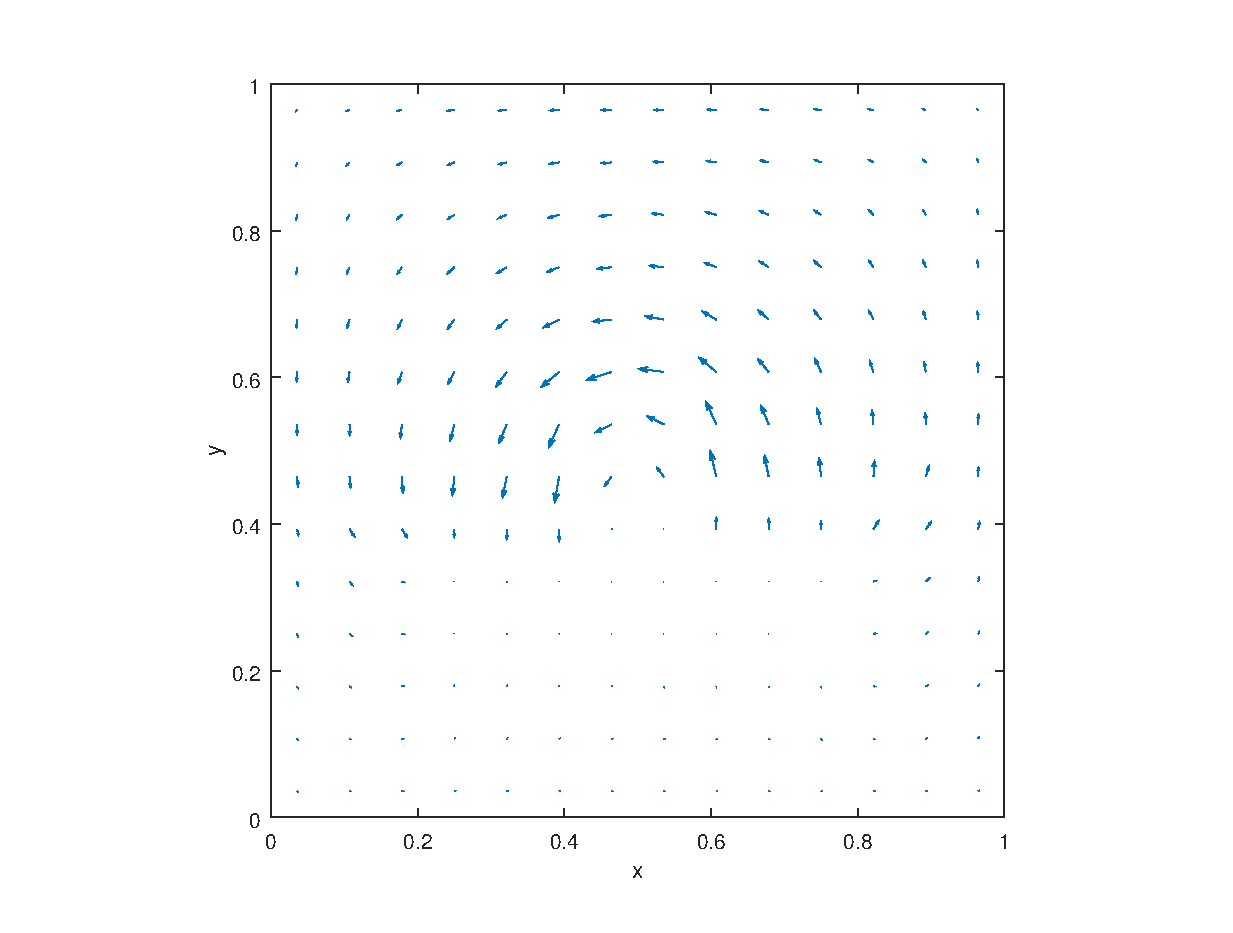
\includegraphics[scale=0.7]{eps/plotMSinhomogen}
\end{center}
\caption{Feldbild eines Linienleiters bei inhomogener Materialverteilung.}
\label{fig:V4.PA10}
\end{figure}


\section{Fazit}

Die Methoden zur Lösung elektrostatischer Probleme lösen eine dem Analytischen sehr ähnliche Potentialgleichung. Diese bietet die Möglichkeit, mit nur $N_p$ Unbekannten das elektrostatische Potential und damit auch das $E$- und $D$-Feld für eine große Anzahl an Problemen zu bestimmen. Das kompliziertere Beispiel zeigt auf, dass analytisch nicht lösbare Probleme mit dem Verfahren gut approximiert werden können, wobei das Ergebnis bereits bei recht wenigen Stützstellen eine gute Näherung bietet. 
%%%%% Teilfazit zur Magnetostatik %%%
Die Verfahren zur Skalaren Magnetostatik in 2D bestätigen anschaulich die Erwartungen von physikalischen Feldbildern und liefern schon bei der verwendeten, relativ geringen Anzahl an Stützstellen ein qualitativ aussagekräftiges Bild. Hiermit wird anschaulich belegt, dass der Ansatz eines Skalarpotentials für das magnetische Feld verbunden mit den unphysikalischen magnetischen Ladungen $q_m$ als Hilfsgrößen einen eleganten und und verglichem mit einem Vektorpotentialansatz auch einfachereren Weg bietet.

\newpage
\newpage

\section{Matlab-Code}
\label{appendix}

\subsection{Code zu Aufgabe 1}
\label{code4.1}
\textit{ Aufgabe siehe Seite \pageref{v4.PA.1} }
\lstinputlisting[language=Octave]{../../code_main/versuch4/solveES.m}

\subsection{Code zu Aufgabe 2}
\label{code4.2}
\textit{Aufgabe siehe Seite \pageref{v4.PA.2} }
\lstinputlisting[language=Octave]{../../code_main/versuch4/calcCap.m}

\subsection{Code zu Aufgabe 3}
\label{code4.3}
\textit{Aufgabe siehe Seite \pageref{v4.PA.3}}
\lstinputlisting[language=Octave]{../../code_main/versuch4/exampleCaps.m}

%\subsection{Code zu Aufgabe 4}
%\label{code4.4}
%\textit{siehe Sektion \ref{code4.3}}

\subsection{Code zu Aufgabe 5}
\label{code4.5}
\textit{Aufgabe siehe Seite \pageref{v4.PA.5}}
\lstinputlisting[language=Octave]{../../code_main/versuch4/plotConv.m}

\subsection{Code zu Aufgabe 6}
\label{code4.6}
\textit{Aufgabe siehe Seite \pageref{v4.PA.6}}
\lstinputlisting[language=Octave]{../../code_main/versuch4/plotConvCap.m}

\subsection{Code zu Aufgabe 7}
\label{code4.7}
\textit{Aufgabe siehe Seite \pageref{v4.PA.7}}
\lstinputlisting[language=Octave]{../../code_main/versuch4/exampleHi.m}

\subsection{Code zu Aufgabe 8}
\label{code4.8}
\textit{Aufgabe siehe Seite \pageref{v4.PA.8}}
\lstinputlisting[language=Octave]{../../code_main/versuch4/solveMS.m}

\subsection{Code zu Aufgabe 9}
\label{code4.9}
\textit{Aufgabe siehe Seite \pageref{v4.PA.9}}
\lstinputlisting[language=Octave]{../../code_main/versuch4/exampleMShomogen.m}

\subsection{Code zu Aufgabe 10}
\label{code4.10}
\textit{Aufgabe siehe Seite \pageref{v4.PA.10}}
\lstinputlisting[language=Octave]{../../code_main/versuch4/exampleMSinhomogen.m}

\end{document}